\chapter{Evil Twin Attack Simulation}

This chapter presents the simulation of an Evil Twin attack, demonstrating the steps required to create a malicious network mimicking a legitimate access point (AP). The Evil Twin attack is commonly used to deceive users into connecting to a rogue network controlled by an attacker. This simulation focuses on setting up the Evil Twin network, with the limitation of having only one wireless network interface card (NIC). For a complete attack, two NICs are required: one to create the rogue AP and the other to perform DNS routing.

\section{Introduction to Evil Twin Attacks}
An Evil Twin attack involves creating a fake wireless AP with the same ESSID as the target network. This rogue network can be used to intercept user traffic, steal credentials, or inject malicious payloads. In this simulation, the focus is on creating the fake AP and executing a deauthentication attack to disconnect devices from the legitimate network, enticing them to connect to the Evil Twin.

\subsection{Tools and Software Utilized}
The following tools were utilized during the simulation:

\begin{itemize}
    \item \textbf{Airmon-ng}: To enable monitor mode on the wireless adapter.
    \item \textbf{Airodump-ng}: To scan for nearby networks and identify the target ESSID and channel.
    \item \textbf{Airbase-ng}: To create the Evil Twin network.
    \item \textbf{Aireplay-ng}: To execute the deauthentication attack.
\end{itemize}

\section{Objective and Methodology}
The objective of this simulation is to emulate an Evil Twin attack by creating a rogue network and demonstrating its visibility to nearby devices. The following steps outline the methodology:

\begin{enumerate}
    \item \textbf{Switching to Monitor Mode:} The first step involves enabling monitor mode on the wireless adapter. This allows the adapter to capture all wireless traffic in range. The command \texttt{sudo airmon-ng start wlan0} was used to switch the adapter from managed mode to monitor mode. Figure \ref{fig:monitor_mode} shows the output of this command.
    
    \begin{figure}[h!]
        \centering
        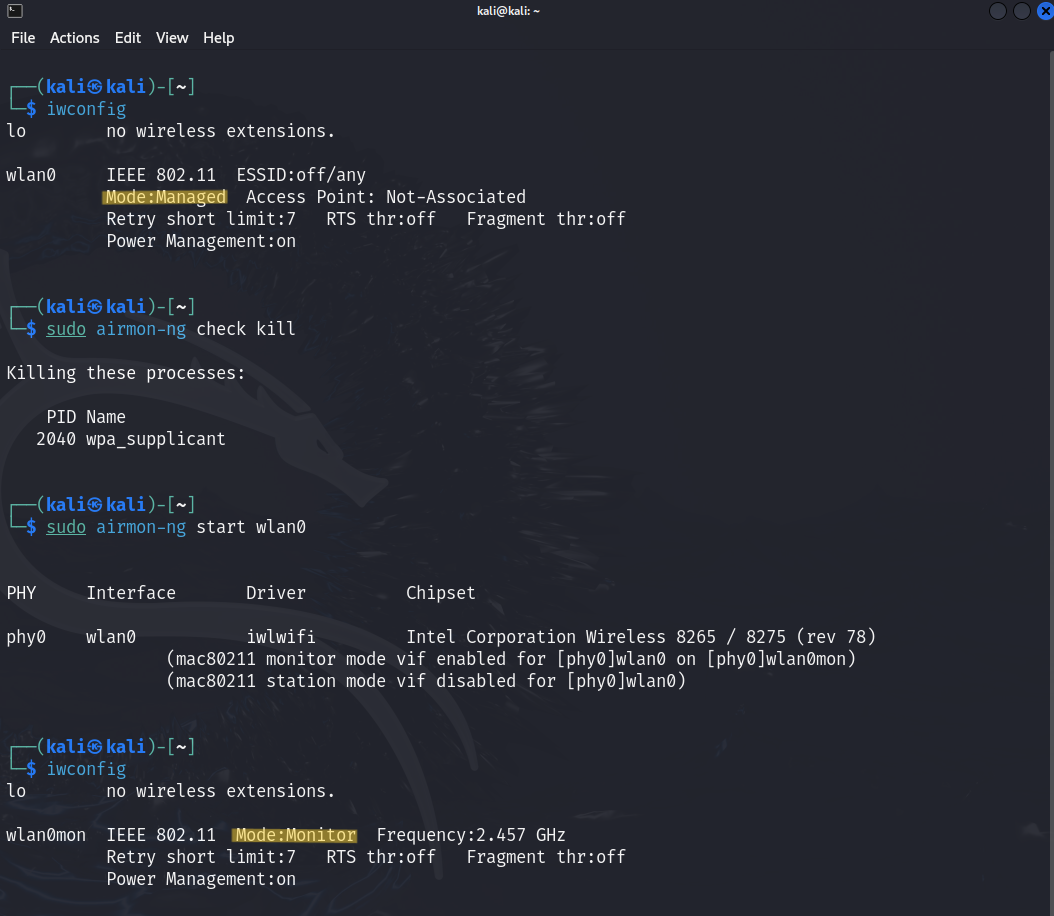
\includegraphics[width=0.8\linewidth]{images/wlanmon.png}
        \caption{Switching the network interface to monitor mode.}
        \label{fig:monitor_mode}
    \end{figure}

    \item \textbf{Scanning for Nearby Networks:} Using the \texttt{sudo airodump-ng wlan0mon} command, nearby wireless networks were scanned to identify the target network. The scan revealed the ESSID and channel of the target network, as shown in Figure \ref{fig:network_scan}.
    
    \begin{figure}[h!]
        \centering
        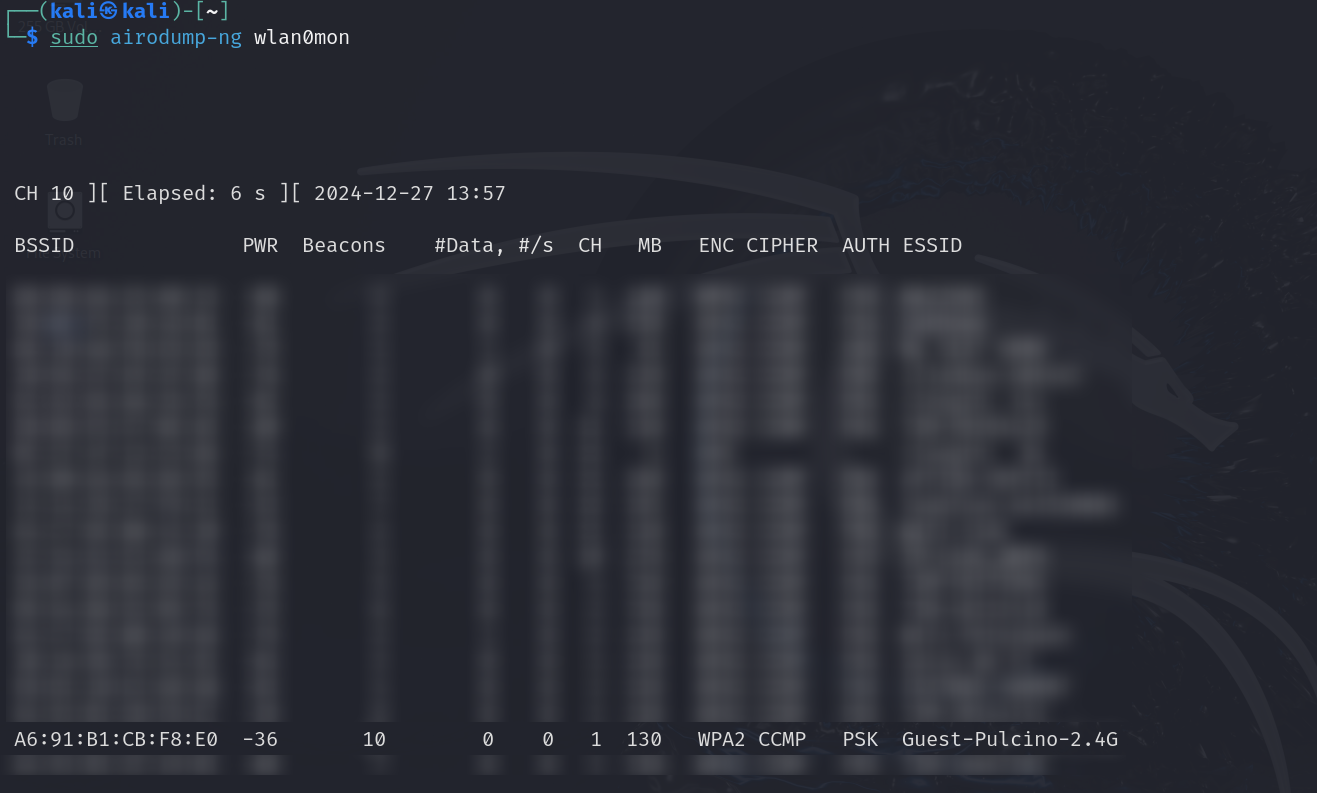
\includegraphics[width=0.8\linewidth]{images/networklist2.png}
        \caption{Scanning nearby networks to identify the target.}
        \label{fig:network_scan}
    \end{figure}

    \item \textbf{Creating the Evil Twin Network:} With the target network's ESSID and channel identified, the Evil Twin network was created using the following command: 
    \texttt{sudo airbase-ng -e TargetESSID -c Channel wlan0mon}. 
    The command output, displayed in Figure \ref{fig:evil_twin_creation}, confirms the successful creation of the rogue AP.
    
    \begin{figure}[h!]
        \centering
        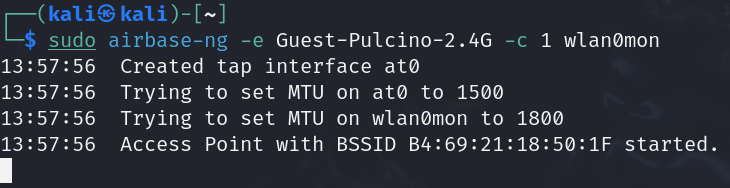
\includegraphics[width=0.8\linewidth]{images/evil_twin_creation.png}
        \caption{Creating the Evil Twin network with Airbase-ng.}
        \label{fig:evil_twin_creation}
    \end{figure}

    \item \textbf{Deauthentication Attack:} To disconnect clients from the legitimate network and prompt them to connect to the Evil Twin, a deauthentication attack was executed using the command:
    \texttt{sudo aireplay-ng --deauth 0 -a TargetBSSID wlan0mon}. 
    The process, as shown in Figure \ref{fig:deauth_attack}, involves sending deauthentication frames to all devices connected to the target network.
    
    \begin{figure}[h!]
        \centering
        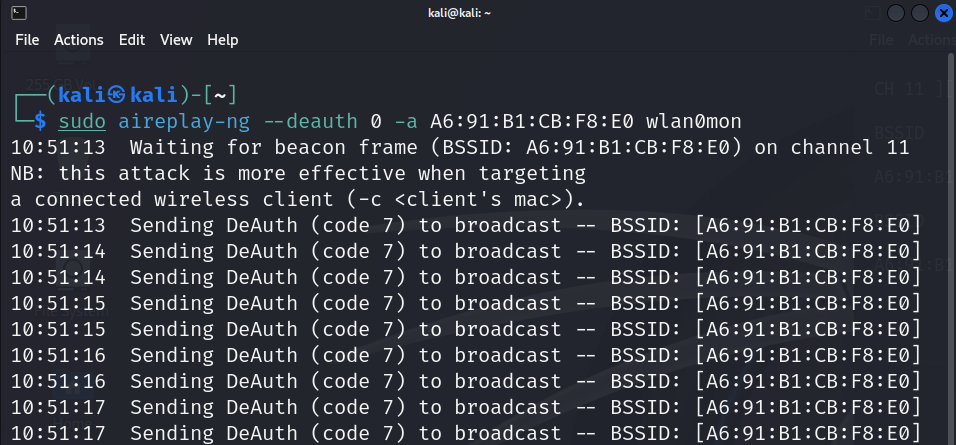
\includegraphics[width=0.8\linewidth]{images/dauth.png}
        \caption{Executing a deauthentication attack.}
        \label{fig:deauth_attack}
    \end{figure}

    \item \textbf{Testing Device Connection:} After the deauthentication attack, a mobile device was used to test the visibility of the Evil Twin network. Figure \ref{fig:device_connection} shows the mobile device successfully connecting to the rogue AP.
    
    \begin{figure}[h!]
        \centering
        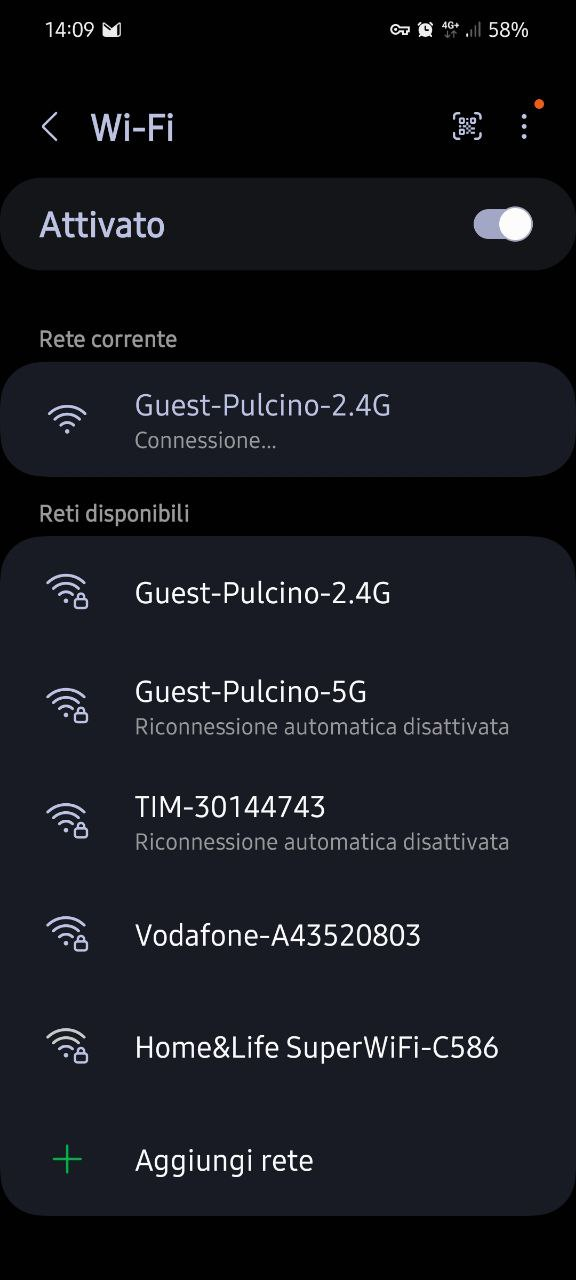
\includegraphics[width=0.5\linewidth]{images/device_connection.jpg}
        \caption{A mobile device connecting to the Evil Twin network.}
        \label{fig:device_connection}
    \end{figure}

    \item \textbf{Confirming the Connection:} The \texttt{airbase-ng} tool confirmed the successful connection of the device to the Evil Twin network, as depicted in Figure \ref{fig:connection_confirmation}.
    
    \begin{figure}[h!]
        \centering
        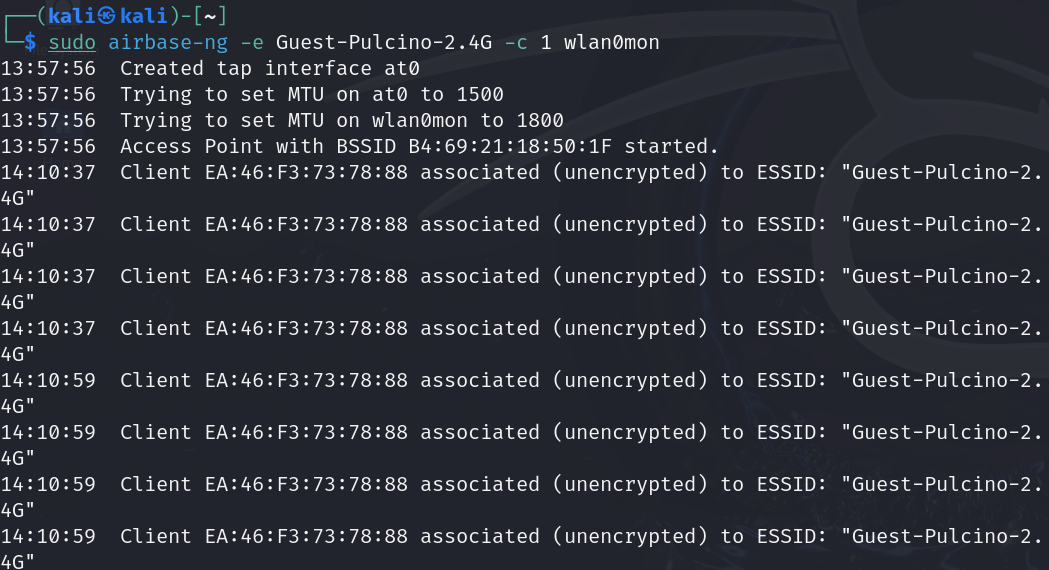
\includegraphics[width=0.8\linewidth]{images/connection_confirmation.png}
        \caption{Connection of the device confirmed by Airbase-ng.}
        \label{fig:connection_confirmation}
    \end{figure}

\end{enumerate}

\section{DNS Routing Configuration (Theoretical)}
To simulate a fully functional Evil Twin attack, DNS routing must be configured to redirect client requests. Although this step was not implemented in the current simulation due to the limitation of having only one NIC, the following commands are provided for completeness:

\begin{enumerate}
    \item Enable IP forwarding:\\
    \textit{echo 1 > /proc/sys/net/ipv4/ip_forward}

    \item Configure iptables for DNS redirection:\\
    \textit{iptables -t nat -A PREROUTING -p udp --dport 53 -j DNAT --to-destination 192.168.1.1}\\
    \textit{iptables -t nat -A POSTROUTING -j MASQUERADE}

    \item Start a DHCP server (e.g., \texttt{dnsmasq}) to assign IP addresses to connected devices.
\end{enumerate}

These commands illustrate the steps required to establish a functional rogue AP capable of routing and handling DNS requests.

\section{Results and Analysis}
The simulation successfully demonstrated the creation of an Evil Twin network and its visibility to nearby devices. The deauthentication attack effectively disconnected clients from the legitimate AP, encouraging them to connect to the rogue network. The results highlight the vulnerabilities of wireless networks to such attacks and the importance of implementing countermeasures, such as enabling WPA3 and monitoring for rogue APs.

\section{Conclusion}
This simulation emphasized the potential risks of Evil Twin attacks, even in a simplified setup. While the absence of DNS routing limited the scope of the attack, the exercise highlighted the ease with which an attacker can create a rogue AP to deceive users.

With the advent of WPA3, some vulnerabilities exploited in Evil Twin attacks have been mitigated. WPA3 introduces robust security features such as the Simultaneous Authentication of Equals (SAE) handshake, which replaces the WPA2 pre-shared key (PSK) authentication method. SAE is resistant to offline dictionary attacks and enhances the security of the authentication process. Additionally, WPA3 mandates the use of Protected Management Frames (PMF), which safeguard management frames like deauthentication and disassociation messages from being spoofed, thereby reducing the efficacy of deauthentication attacks.

However, it is important to note that the Evil Twin attack remains a critical issue regardless of the technology used on the access point. This is because the attack targets the user, not the network itself. Even with WPA3, a rogue AP can mimic a legitimate network’s ESSID and lure users into connecting to it. If a device is not configured to verify the server certificate (as in EAP-TLS or other enterprise-level configurations), users might still fall victim to such attacks. Furthermore, some legacy devices and networks that do not fully support WPA3 features may remain vulnerable.

